\documentclass{article}
    % General document formatting
    \usepackage[margin=0.7in]{geometry}
    \usepackage[parfill]{parskip}
    \usepackage[utf8]{inputenc}
    \usepackage{amsmath}
    \usepackage{amssymb}
    \usepackage{tikz}
    \usepackage{fancyhdr}
    \usepackage{listings}
    \usepackage{multicol}

\pagestyle{fancy}
\fancyhf{}
\rhead{Edgar Jacob Rivera Rios - A01184125}

\begin{document}
\begin{titlepage}

    \newcommand{\HRule}{\rule{\linewidth}{0.5mm}} % Defines a new command for the horizontal lines, change thickness here

    \center % Center everything on the page

    %----------------------------------------------------------------------------------------
    %	HEADING SECTIONS
    %----------------------------------------------------------------------------------------

    \textsc{\LARGE Tecnológico de Monterrey}\\[1.5cm] % Name of your university/college
    \textsc{\Large Computational intelligence}\\[0.5cm] % Major heading such as course name
    %\textsc{\large Minor Heading}\\[0.5cm] % Minor heading such as course title

    %----------------------------------------------------------------------------------------
    %	TITLE SECTION
    %----------------------------------------------------------------------------------------

    \HRule \\[0.4cm]
    { \huge \bfseries Homework 4}\\[0.4cm] % Title of your document
    \HRule \\[1.5cm]

    %----------------------------------------------------------------------------------------
    %	AUTHOR SECTION
    %----------------------------------------------------------------------------------------

    \begin{minipage}{0.4\textwidth}
    \begin{flushleft} \large
    \emph{Student:}\\
    Jacob \textsc{Rivera} % Your name
    \end{flushleft}
    \end{minipage}
    ~
    \begin{minipage}{0.4\textwidth}
    \begin{flushright} \large
    \emph{Professor:} \\
    Dr. José Carlos \textsc{Bayliss} % Supervisor's Name
    \end{flushright}
    \end{minipage}\\[2cm]

    % If you don't want a supervisor, uncomment the two lines below and remove the section above
    %\Large \emph{Author:}\\
    %John \textsc{Smith}\\[3cm] % Your name

    %----------------------------------------------------------------------------------------
    %	DATE SECTION
    %----------------------------------------------------------------------------------------

    {\large \today}\\[2cm] % Date, change the \today to a set date if you want to be precise

    %----------------------------------------------------------------------------------------
    %	LOGO SECTION
    %----------------------------------------------------------------------------------------

    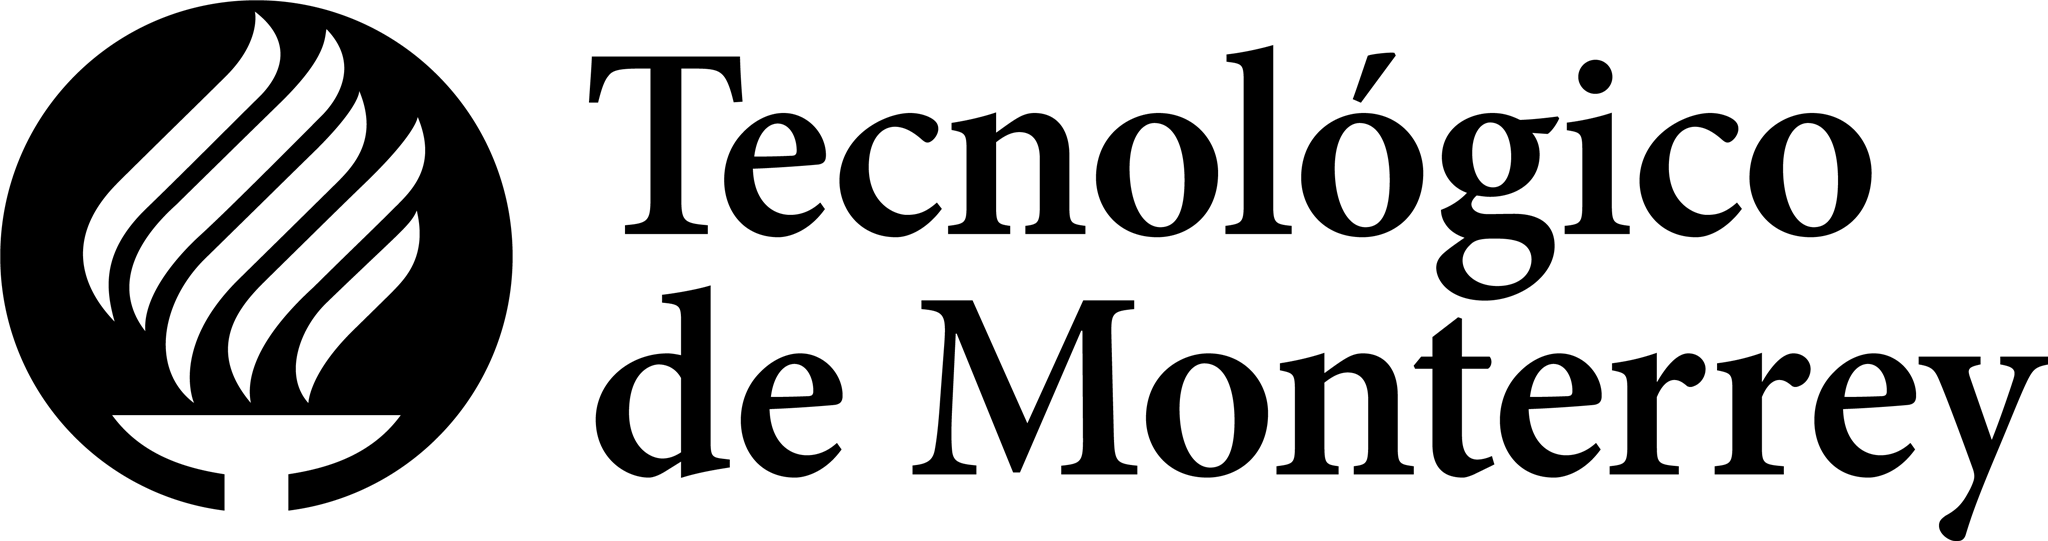
\includegraphics[width=0.4\textwidth,height=\textheight,keepaspectratio]{../Assets/logo-tec-negro.png} % Include a department/university logo - this will require the graphicx package

    %----------------------------------------------------------------------------------------

    \vfill % Fill the rest of the page with whitespace

\end{titlepage}
\section*{Problems}
\begin{enumerate}
    \item Tournament selection
    \begin{table}[h]
        \centering
        \begin{tabular}{l|l|l}
            & Population & $f$ \\
            \hline
            A & 010111000  & -1 \\
            B & 011101001  & 4 \\
            C & 111000110  & -2 \\
            D & 100001000  & 1 \\
            E & 010101000  & 0
        \end{tabular}
    \end{table}
    \begin{itemize}
        \item How many copies of each chromosome are present in the mating pool?
        \begin{itemize}
            \item A: 0
            \item B: 3
            \item C: 0
            \item D: 2
            \item E: 0
        \end{itemize}
        \item What is the average fitness of the chromosomes in the mating pool?

        2.8

        \item If the tournament size is reduced to one, what is the probability that the chromosome 100001000 appears in the mating pool?

        100\%

        \item If the tournament size is increased to five, and both crossover and mutation rate are set to zero, what is the probability that the chromosome 010111000 survives to the next population?

        0\%

    \end{itemize}

    \item Whole arithmetic crossover
    \begin{align*}
        x=\{ 0.18, 0.75, 0.92, 0.26, 0.44 \}\\
        y=\{ 0.36, 0.77, 0.62, 0.13, 0.51 \}\\
    \end{align*}
    \begin{align*}
        c^{1}_{.5} &= \{ 0.27, .76, .77, .195, .475 \} & c^{2}_{.5} &= \{ 0.27, .76, .77, .195, .475 \}\\
        c^1_{.1} &= \{ 0.342, 0.768, 0.65, 0.143 ,0.503 \} & c^2_{.1} &= \{ 0.198, 0.752, 0.89, 0.247 ,0.447\}\\
    \end{align*}

    \pagebreak
    \item Exponential ranking selection
    \begin{table}[h]
        \centering
        \begin{tabular}{l|l|l|l|l}
            & Population & $f$ & r & $f'$ \\
            \hline
            A & 6661166703  & 5 & 3.5 & 2.296875\\
            B & 3306772232  & 5 & 3.5 & 2.296875\\
            C & 0489794549  & 4 & 1.5 & 0.421875\\
            D & 2660088784  & 4 & 1.5 & 0.421875\\
            E & 3578647359  & 3 & 0 & 0
        \end{tabular}
    \end{table}
    Sum: 5.4375
    \begin{itemize}
        \item A: $\frac{2.29}{5.4375} = 0.4224$
        \item B: $\frac{2.29}{5.4375} = 0.4224$
        \item C: $\frac{0.42}{5.4375} = 0.0775$
        \item D: $\frac{0.42}{5.4375} = 0.0775$
        \item E: 0
    \end{itemize}


    \item Schemata
    \begin{itemize}
        \item Given two schemata, 1*001*1* and 00*11*11, which schema corresponds to more solutions?
        \begin{multicols}{2}
            1*001*1* $\rightarrow$ 8
            \begin{itemize}
                \item 11001111
                \item 11001110
                \item 11001011
                \item 11001010
                \item 10001111
                \item 10001110
                \item 10001011
                \item 10001010
            \end{itemize}
            \columnbreak
            00*11*11 $\rightarrow$ 4
            \begin{itemize}
                \item 00111111
                \item 00111011
                \item 00011111
                \item 00011011
            \end{itemize}
        \end{multicols}
        \item What is the order of the schemata 01101001, ****1**0 and 1*0*0010?
        \begin{itemize}
            \item 01101001 $\rightarrow$ 8 $\rightarrow$ 2
            \item ****1**0 $\rightarrow$ 2 $\rightarrow$ 0
            \item 1*0*0010 $\rightarrow$ 6 $\rightarrow$ 1
        \end{itemize}
        \item What is the defining length of the schemata 00**1010, **0**111 and *0***1*0?
        \begin{itemize}
            \item 00**1010 $\rightarrow$ 7
            \item **0**111 $\rightarrow$ 5
            \item *0***1*0 $\rightarrow$ 6
        \end{itemize}

        \pagebreak

        \item Given a population of five chromosomes: 100, 001, 111, 010, and 000, how many different schemata exist in such a population?  As part of your answer, calculate the lower and upper bounds of schemata in the population.\\
        Upper bound = $5*2^3 = 40$ \\
        Lower bound = $2^3 = 8$\\
        \begin{multicols}{4}
            \begin{itemize}
                \item 000
                \item 00*
                \item 0*0
                \item *00
                \item 0**
                \item **0
                \item *0*
                \item ***
                \item 010
                \item 01*
                \item *10
                \item *1*
                \item 111
                \item 11*
                \item 1*1
                \item *11
                \item 1**
                \item **1
                \item 001
                \item 0*1
                \item *01
                \item 100
                \item 10*
                \item 1*0
            \end{itemize}
        \end{multicols}
    \end{itemize}

    \item Practical case

    The representation chosen for this exervise would be one in which each action is represented by a number associated with it. For example 1 = Go Up, 2 = Go Right, 3 = Go Down and 4 = Go Left. As the memory of the robot can only store 100 actions, the chromosome would have a length of 100. A crossover operator would be as simple as an index in which each parent splits and each part goes to each children. A mutation operand would simply change a selected entity to a random option different that the one it already has.

    The optimal path in the figure shown, which consists in actions “move up”, “move to the right”, “move to the right”, “move to the right”, “move up”, “move up”, “move to the left”, “move to the left”, “move to the left”, “move up”, and “move up”  would then be represented as $[1,2,2,2,1,1,3,3,3,1,1 ... 1]$

    \item Analysis
    \begin{itemize}
        \item What would you think of using elitism in a steady-state genetic algorithm? Do you think it is a good idea? What would be the benefits?

        Elitism may be beneficial when you reach a steady-state, because you can replace more of your population and maybe found a better solution and breaking with the steady-state. Although if the population is already too uniform, it probably won't have a significant impact in creating different items in the new population.

        \item Imagine that someone proposes a mutation operator for binary strings that is inspired on a uniform crossover. This mutation operator uses a binary template and only the elements located at positions of the template that contain a 1 will be flipped. What could you say about this mutation operator?

        It may be useful, but as only that positions change it may lead to a somewhat static set of chromosomes which the would need to be mutated more to create more variety in the new populations.

        \item Imagine that linear ranking selection (using C = 2) is executed on a population of $n$ chromosomes. What would be the effect on the selection probabilities if the fitness of every chromosome in the population is multiplied by a constant $k$?

        The rank would remain the same as the constant is applied to all, in any case, if the constant is less than 1, the points would be drawn closer together, whereas if the constant is bigger than one, the ranks would be spread farther away.

        \item Given a binary-string chromosome of 100 genes and a mutation rate $pm = 0.01$ (that is evaluated independently for each gene in the chromosome), what is the probability that a given chromosome  remains unaltered during the mutation phase? What would be the probability that a given chromosome remains unaltered during the mutation phase if $pm = 0.05$? What value should we use for pm if we would like that around half of the genes in the chromosomes are flipped as a result of mutation?

        If the $pm$ is equal to 0.01, that means that the possibility of remain the same, would be calculated by the expression $1 - pm$, which would then be equivalent to 0.99 in this case. On the other hand, if $pm$ is equal to 0.05, the probability of remaining the same would then be 0.95. In order to have half the chromosomes flipped, you would then have to have a $pm$ of 0.5.

        \item Given two real-valued chromosomes of length five, $\vec{x} = {x_1, x_2, x_3, x_4, x_5}$ and $\vec{y} = {y_1, y_2, y_3, y_4, y_5}$, what would be the result of combining $\vec{x}$ and $\vec{y}$ through a whole arithmetic crossover with $\alpha$ = 1.0? How would the offspring change if $\alpha$ = 0?

        The result of combining $\vec{x}$ and $\vec{y}$ with and $\alpha$ of 1 would be just the same as $\vec{x}$ and $\vec{y}$ because the values in $\vec{y}$ would be mutliplied by 0 in the first instance and the values of $\vec{x}$ in the second. If $\alpha$ is set to 0,the same would pass, only the positions would be changed.

    \end{itemize}

\end{enumerate}
\end{document}